% Practice Test 18 — Florida Edition
% Questions: 30 (26 MC + 4 SA)
% Generated by scripts/generate_practice_tests.py

\begin{practiceQuestion}{1-3-q12}{mc}
\begin{questionText}
A proportional table has $k = \frac{3}{4}$. Which pair could be in the table?
\end{questionText}
\choiceA{$(8, 10)$}
\choiceB{$(8, 6)$}
\choiceC{$(12, 8)$}
\choiceD{$(4, 2)$}
\correctAnswer{B}
\explanation{If $k = \frac{3}{4}$, then $y = \frac{3}{4}x$. For $x = 8$: $y = \frac{3}{4} \times 8 = 6$. So $(8, 6)$ works.}
\end{practiceQuestion}

\begin{practiceQuestion}{1-6-q04}{mc}
\begin{questionText}
A recipe for $4$ people uses $\frac{3}{2}$ cups of rice. How much rice is needed for $10$ people?
\end{questionText}
\choiceA{$2\frac{1}{2}$ cups}
\choiceB{$3$ cups}
\choiceC{$3\frac{3}{4}$ cups}
\choiceD{$5$ cups}
\correctAnswer{C}
\explanation{Per person: $\frac{3}{2} \div 4 = \frac{3}{8}$ cup. For $10$: $\frac{3}{8} \times 10 = \frac{30}{8} = 3\frac{3}{4}$ cups.}
\end{practiceQuestion}

\begin{practiceQuestion}{2-1-q12}{mc}
\begin{questionText}
$63$ is $90\%$ of what number?
\end{questionText}
\choiceA{$56.7$}
\choiceB{$67$}
\choiceC{$70$}
\choiceD{$72$}
\correctAnswer{C}
\explanation{Divide: $63 \div 0.90 = 70$.}
\end{practiceQuestion}

\begin{practiceQuestion}{2-2-q12}{mc}
\begin{questionText}
Sarah and Jake both solve ``What is $40\%$ of $75$?'' Sarah uses a proportion; Jake uses an equation. Which statement is true?
\end{questionText}
\choiceA{Only the proportion method works}
\choiceB{Only the equation method works}
\choiceC{Both methods give the same answer}
\choiceD{The methods give different answers}
\correctAnswer{C}
\explanation{Proportion: $\frac{n}{75} = \frac{40}{100}$ gives $n = 30$. Equation: $n = 0.40 \times 75 = 30$. Both give $30$.}
\end{practiceQuestion}

\begin{practiceQuestion}{2-6-q11}{mc}
\begin{questionText}
What is the simple interest on $\$1{,}200$ at $3.5\%$ for $2$ years?
\end{questionText}
\choiceA{$\$42$}
\choiceB{$\$72$}
\choiceC{$\$84$}
\choiceD{$\$210$}
\correctAnswer{C}
\explanation{$I = 1{,}200 \times 0.035 \times 2 = \$84$.}
\end{practiceQuestion}

\begin{practiceQuestion}{2-7-q02}{mc}
\begin{questionText}
A student measured a table as $4.5$ feet long. The actual length is $5$ feet. What is the percent error?
\end{questionText}
\choiceA{$0.5\%$}
\choiceB{$5\%$}
\choiceC{$10\%$}
\choiceD{$11.1\%$}
\correctAnswer{C}
\explanation{$\frac{|4.5 - 5|}{5} \times 100 = \frac{0.5}{5} \times 100 = 10\%$.}
\end{practiceQuestion}

\begin{practiceQuestion}{3-2-q13}{mc}
\begin{questionText}
A bank account has $-\$50$ (overdrawn). A deposit of $\$75$ is made. What is the new balance?
\end{questionText}
\choiceA{$-\$125$}
\choiceB{$-\$25$}
\choiceC{$\$25$}
\choiceD{$\$125$}
\correctAnswer{C}
\explanation{$(-50) + 75 = 25$. The deposit is larger than the overdraft, so the balance becomes positive.}
\end{practiceQuestion}

\begin{practiceQuestion}{3-3-q03}{mc}
\begin{questionText}
Which expression is equivalent to $(-5) - 3$?
\end{questionText}
\choiceA{$(-5) + 3$}
\choiceB{$(-5) + (-3)$}
\choiceC{$5 + 3$}
\choiceD{$5 + (-3)$}
\correctAnswer{B}
\explanation{Subtraction means adding the opposite: $(-5) - 3 = (-5) + (-3)$.}
\end{practiceQuestion}

\begin{practiceQuestion}{4-4-q14}{mc}
\begin{questionText}
Factor $16x + 24y - 8$.
\end{questionText}
\choiceA{$4(4x + 6y - 2)$}
\choiceB{$8(2x + 3y - 1)$}
\choiceC{$2(8x + 12y - 4)$}
\choiceD{$8(2x + 3y + 1)$}
\correctAnswer{B}
\explanation{GCF of $16$, $24$, and $8$ is $8$. Divide each: $16x \div 8 = 2x$, $24y \div 8 = 3y$, $-8 \div 8 = -1$. Result: $8(2x + 3y - 1)$.}
\end{practiceQuestion}

\begin{practiceQuestion}{4-5-q12}{mc}
\begin{questionText}
Simplify $(3.5n - 2.1) - (1.5n + 0.9)$.
\end{questionText}
\choiceA{$2n - 3$}
\choiceB{$5n - 3$}
\choiceC{$2n - 1.2$}
\choiceD{$2n + 3$}
\correctAnswer{A}
\explanation{Distribute: $3.5n - 2.1 - 1.5n - 0.9$. Combine: $(3.5n - 1.5n) + (-2.1 - 0.9) = 2n - 3$.}
\end{practiceQuestion}

\begin{practiceQuestion}{5-3-q11}{mc}
\begin{questionText}
A student solved $3(x + 4) = 30$ and wrote: $3x + 4 = 30$, $3x = 26$, $x = \frac{26}{3}$. What was the student's error?
\end{questionText}
\choiceA{Divided by $3$ instead of subtracting}
\choiceB{Did not distribute $3$ to the $4$}
\choiceC{Subtracted $4$ from the wrong side}
\choiceD{Forgot to check the answer}
\correctAnswer{B}
\explanation{The student wrote $3x + 4$ instead of $3x + 12$. Distributing correctly gives $3x + 12 = 30$.}
\end{practiceQuestion}

\begin{practiceQuestion}{5-4-q25}{sa}
\begin{questionText}
Solve $2.5x - 7.5 = 10$.
\end{questionText}
\correctAnswer{$x = 7$}
\explanation{Add $7.5$: $2.5x = 17.5$. Divide by $2.5$: $x = 7$. Check: $2.5(7) - 7.5 = 17.5 - 7.5 = 10$ \checkmark.}
\end{practiceQuestion}

\begin{practiceQuestion}{5-5-q06}{mc}
\begin{questionText}
Solve $-4x > 20$.
\end{questionText}
\choiceA{$x > -5$}
\choiceB{$x < -5$}
\choiceC{$x > 5$}
\choiceD{$x < 5$}
\correctAnswer{B}
\explanation{Divide by $-4$ and flip the sign: $x < -5$.}
\end{practiceQuestion}

\begin{practiceQuestion}{5-6-q20}{sa}
\begin{questionText}
Solve $-5x + 15 \geq 30$. Describe the graph.
\end{questionText}
\correctAnswer{$x \leq -3$; closed circle at $-3$, shade left}
\explanation{Subtract $15$: $-5x \geq 15$. Divide by $-5$ and flip: $x \leq -3$. Closed circle at $-3$, shade left.}
\end{practiceQuestion}

\begin{practiceQuestion}{6-2-q14}{mc}
\begin{questionText}
Original scale: $1$ cm $= 10$ m. New scale: $1$ cm $= 40$ m. What is the scale ratio?
\end{questionText}
\choiceA{$\frac{1}{4}$}
\choiceB{$4$}
\choiceC{$30$}
\choiceD{$\frac{1}{30}$}
\correctAnswer{A}
\explanation{Scale ratio: $\frac{10}{40} = \frac{1}{4}$. Every old length is multiplied by $\frac{1}{4}$ on the new drawing.}
\end{practiceQuestion}

\begin{practiceQuestion}{6-4-q17}{mc}
\begin{questionText}
Two angles of a triangle are $25°$ and $25°$. The triangle is:
\end{questionText}
\choiceA{Equilateral}
\choiceB{Isosceles}
\choiceC{Scalene}
\choiceD{Impossible}
\correctAnswer{B}
\explanation{Third angle: $180° - 25° - 25° = 130°$. Two equal angles means two equal sides, making it isosceles.}
\end{practiceQuestion}

\begin{practiceQuestion}{6-5-q27}{gmc}
\begin{questionText}
The diagram shows a cone being sliced. Which cut produces a circular cross-section?

\begin{center}
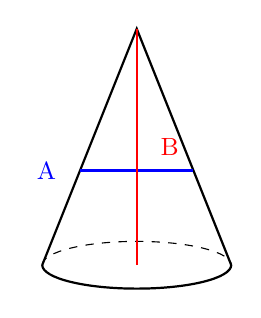
\begin{tikzpicture}[scale=0.6]
  % Cone
  \draw[thick] (-2,0) -- (0,5) -- (2,0);
  \draw[thick] (-2,0) arc[start angle=180,end angle=360,x radius=2,y radius=0.5];
  \draw[dashed] (-2,0) arc[start angle=180,end angle=0,x radius=2,y radius=0.5];
  % Cut A - horizontal
  \draw[thick,blue] (-1.2,2) -- (1.2,2);
  \node[left,blue] at (-1.5,2) {\small A};
  % Cut B - vertical through apex
  \draw[thick,red] (0,0) -- (0,5);
  \node[right,red] at (0.3,2.5) {\small B};
\end{tikzpicture}
\end{center}
\end{questionText}
\choiceA{Cut A (horizontal)}
\choiceB{Cut B (vertical through apex)}
\choiceC{Both cuts}
\choiceD{Neither cut}
\correctAnswer{A}
\explanation{Cut A (horizontal, parallel to the base) produces a circle. Cut B (vertical through the apex) produces a triangle.}
\end{practiceQuestion}

\begin{practiceQuestion}{6-6-q09}{mc}
\begin{questionText}
An angle is $4$ times its supplement. What is the angle?
\end{questionText}
\choiceA{$36°$}
\choiceB{$45°$}
\choiceC{$120°$}
\choiceD{$144°$}
\correctAnswer{D}
\explanation{Let the supplement be $x$. The angle is $4x$. Sum: $x + 4x = 180$. So $5x = 180$ and $x = 36°$. The angle: $4(36) = 144°$.}
\end{practiceQuestion}

\begin{practiceQuestion}{7-1-q17}{mc}
\begin{questionText}
Which of the following is NOT a part of a circle?
\end{questionText}
\choiceA{Center}
\choiceB{Radius}
\choiceC{Vertex}
\choiceD{Diameter}
\correctAnswer{C}
\explanation{A vertex is a corner point found on polygons, not circles. Center, radius, and diameter are all parts of a circle.}
\end{practiceQuestion}

\begin{practiceQuestion}{7-5-q11}{mc}
\begin{questionText}
A cereal box is $30$ cm tall, $20$ cm wide, and $6$ cm deep. What is its surface area?
\end{questionText}
\choiceA{$1{,}440$ cm$^2$}
\choiceB{$1{,}560$ cm$^2$}
\choiceC{$1{,}800$ cm$^2$}
\choiceD{$3{,}600$ cm$^2$}
\correctAnswer{C}
\explanation{$SA = 2(30 \times 20) + 2(30 \times 6) + 2(20 \times 6) = 1200 + 360 + 240 = 1{,}800$ cm$^2$.}
\end{practiceQuestion}

\begin{practiceQuestion}{7-6-q16}{mc}
\begin{questionText}
A rectangular prism has a volume of $240$ cm$^3$. Its base is $8$ cm by $6$ cm. What is the height?
\end{questionText}
\choiceA{$4$ cm}
\choiceB{$5$ cm}
\choiceC{$6$ cm}
\choiceD{$10$ cm}
\correctAnswer{B}
\explanation{$B = 8 \times 6 = 48$ cm$^2$. $h = V \div B = 240 \div 48 = 5$ cm.}
\end{practiceQuestion}

\begin{practiceQuestion}{7-7-q29}{gsa}
\begin{questionText}
A cylindrical can is shown. Find the surface area of the can. Use $\pi \approx 3.14$.

\begin{center}
\begin{tikzpicture}[scale=0.3]
  \draw[thick,funBlue,fill=funBlue!10] (-3,0) -- (-3,10) arc (180:360:3 and 1) -- (3,0) arc (0:180:3 and 1);
  \draw[thick,funBlue,fill=funBlue!20] (0,10) ellipse (3 and 1);
  \draw[thick,dashed,funBlue] (-3,0) arc (180:360:3 and 1);
  \draw[thick,funRed,<->] (4.5,0) -- (4.5,10);
  \node[right,funRed] at (4.5,5) {$10$ cm};
  \draw[thick,funRed,<->] (-3,-2) -- (3,-2);
  \node[below,funRed] at (0,-2) {$d = 6$ cm};
\end{tikzpicture}
\end{center}
\end{questionText}
\correctAnswer{$244.92$ cm$^2$}
\explanation{$r = 3$ cm. $SA = 2\pi r^2 + 2\pi rh = 2(3.14)(9) + 2(3.14)(3)(10) = 56.52 + 188.4 = 244.92$ cm$^2$.}
\end{practiceQuestion}

\begin{practiceQuestion}{8-1-q18}{mc}
\begin{questionText}
A poll found that $35\%$ of a random sample of $400$ students prefer pizza for lunch. Which statement is the best inference?
\end{questionText}
\choiceA{Exactly $35\%$ of all students prefer pizza}
\choiceB{About $35\%$ of the entire student population likely prefers pizza}
\choiceC{No students prefer anything other than pizza}
\choiceD{The poll is invalid because not all students were surveyed}
\correctAnswer{B}
\explanation{A random sample provides an estimate. About $35\%$ of the population likely prefers pizza, but the exact percentage may differ slightly.}
\end{practiceQuestion}

\begin{practiceQuestion}{8-3-q12}{mc}
\begin{questionText}
When is a dot plot a better choice than a box plot for comparing two groups?
\end{questionText}
\choiceA{When data sets are very large}
\choiceB{When you want to see every individual data point}
\choiceC{When you only want to compare medians}
\choiceD{When the data is categorical}
\correctAnswer{B}
\explanation{Dot plots show every data point, which is useful for small data sets where individual values matter.}
\end{practiceQuestion}

\begin{practiceQuestion}{8-4-q18}{mc}
\begin{questionText}
Class A: median $85$, IQR $8$, range $20$. Class B: median $80$, IQR $15$, range $40$. A student says ``Class B is better because it has a wider range.'' Is the student correct?
\end{questionText}
\choiceA{Yes — wider range means more talent}
\choiceB{No — wider range means less consistency, and Class A has a higher median}
\choiceC{Yes — Class B's scores spread more, which is always better}
\choiceD{No — range does not measure anything useful}
\correctAnswer{B}
\explanation{A wider range indicates more variability, not better performance. Class A has a higher median and is more consistent (smaller IQR and range).}
\end{practiceQuestion}

\begin{practiceQuestion}{8-5-q22}{sa}
\begin{questionText}
How many data values are shown in this stem-and-leaf plot?

Stem $5$: $1\;\;3\;\;5$ \quad Stem $6$: $0\;\;2\;\;4\;\;7\;\;8$ \quad Stem $7$: $1\;\;6$ \quad Stem $8$: $0$
\end{questionText}
\correctAnswer{$11$}
\explanation{Count leaves: $3 + 5 + 2 + 1 = 11$.}
\end{practiceQuestion}

\begin{practiceQuestion}{8-6-q18}{mc}
\begin{questionText}
Two circle graphs compare how Class A and Class B spend their free time. Class A shows $45\%$ on sports; Class B shows $30\%$ on sports. If Class A has $20$ students and Class B has $30$ students, how many more students in Class B play sports than in Class A?
\end{questionText}
\choiceA{$0$ — the same number}
\choiceB{$9$ is more in Class B}
\choiceC{$3$ is more in Class A}
\choiceD{$1$ more in Class A}
\correctAnswer{A}
\explanation{Class A: $45\%$ of $20 = 9$. Class B: $30\%$ of $30 = 9$. Same number: $9$ each.}
\end{practiceQuestion}

\begin{practiceQuestion}{9-4-q03}{mc}
\begin{questionText}
A bag contains $4$ red marbles and $1$ blue marble. Which type of probability model does this represent?
\end{questionText}
\choiceA{Uniform}
\choiceB{Non-uniform}
\choiceC{Both uniform and non-uniform}
\choiceD{Neither}
\correctAnswer{B}
\explanation{The probability of drawing red ($\frac{4}{5}$) is different from drawing blue ($\frac{1}{5}$), so this is a non-uniform model.}
\end{practiceQuestion}

\begin{practiceQuestion}{9-6-q04}{mc}
\begin{questionText}
Two dice are rolled. What is the probability of getting a sum of $2$?
\end{questionText}
\choiceA{$\frac{1}{6}$}
\choiceB{$\frac{1}{12}$}
\choiceC{$\frac{1}{36}$}
\choiceD{$\frac{2}{36}$}
\correctAnswer{C}
\explanation{The only way to get a sum of $2$ is $(1,1)$. $P = \frac{1}{36}$.}
\end{practiceQuestion}

\begin{practiceQuestion}{9-7-q15}{mc}
\begin{questionText}
You simulate flipping a coin $3$ times and counting how many times all $3$ are heads. In $40$ simulations, all $3$ heads occurs $6$ times. What is the experimental probability?
\end{questionText}
\choiceA{$\frac{6}{40} = 0.15$}
\choiceB{$\frac{1}{8} = 0.125$}
\choiceC{$\frac{3}{40} = 0.075$}
\choiceD{$\frac{6}{120} = 0.05$}
\correctAnswer{A}
\explanation{$P = \frac{6}{40} = 0.15$. The theoretical probability is $\frac{1}{8} = 0.125$, close to the simulation result.}
\end{practiceQuestion}
